\section{Software}

\subsection{Mudanças no escopo}
	Algumas informações e diretrizes do projeto foram modificadas desde a concepção da ideia do projeto de software. A seguir apresentamos as mudanças realizadas no projeto para esta entrega.

\subsubsection{Sistema Interno}
	A principal mudança de escopo na implementação do sistema interno, após refinamento de requisitos, se dá pela remoção do controle e apresentação da pressão interna da caixa transportadora, com isso afeta diretamente os Requisitos Funcionais RF001, RF004, RF006, aos quais são destinados às funções descritas previamente.

\subsubsection{Sistema WEB}
	Assim como o sistema interno, as principais mudanças em relação ao escopo planejado para o webapp se dá pela remoção da apresentação de dados da pressão interna da caixa transportadora, removendo assim o Requisito Funcional RF008.
	Outra mudança de escopo definido durante a implementação do sistema se dá na mudança de controle usuários e seus devidos acessos, ao quais não só “Médicos” serão os usuários do sistema, mas sim definidos 3 tipos de usuários, a serem descritos posteriormente, com isso serão atualizados os Requisitos Funcionais RF011 e RF013.

\begin{table}[H]
\centering
\begin{tabular}{|
>{\columncolor[HTML]{C0C0C0}}l |l|l|l|}
\hline
\textbf{Identificador} & \multicolumn{3}{l|}{RF011}                                                                                                                                                                      \\ \hline
\textbf{Nome}          & \multicolumn{3}{l|}{Cadastrar Usuários}                                                                                                                      \\ \hline
\textbf{Módulo}        & \multicolumn{3}{l|}{Sistema Web}                                                                                                                                                            \\ \hline
\textbf{Versão}        & 2                                             & \cellcolor[HTML]{C0C0C0}\textbf{Prioridade}                                             & Essencial                                             \\ \hline
\textbf{Descrição}     & \multicolumn{3}{l|}{\begin{tabular}[c]{@{}l@{}}O web app deve permitir o cadastro de usuários aos quais irão interagir com o sistema web.\end{tabular}} \\ \hline
\end{tabular}
\caption{Sistema Web - requisito funcional 011}
\label{RF011}
\end{table}

\begin{table}[H]
\centering
\begin{tabular}{|
>{\columncolor[HTML]{C0C0C0}}l |l|l|l|}
\hline
\textbf{Identificador} & \multicolumn{3}{l|}{RF013}                                                                                                                                                                      \\ \hline
\textbf{Nome}          & \multicolumn{3}{l|}{Definir nível de autorização dos usuários}                                                                                                                      \\ \hline
\textbf{Módulo}        & \multicolumn{3}{l|}{Sistema Web}                                                                                                                                                            \\ \hline
\textbf{Versão}        & 2                                             & \cellcolor[HTML]{C0C0C0}\textbf{Prioridade}                                             & Essencial                                             \\ \hline
\textbf{Descrição}     & \multicolumn{3}{l|}{\begin{tabular}[c]{@{}l@{}}O web app deverá possuir um nível de acesso diferenciado para os 3 níveis definidos. Seja eles: Administrador, Transportador e Usuário.\end{tabular}} \\ \hline
\end{tabular}
\caption{Sistema Web - requisito funcional 013}
\label{RF013}
\end{table}

\subsubsection{Arquitetura de Software}

Em relação à Arquitetura de Software proposta não houve mudanças de escopo. 
A arquitetura implementada consiste no modelo cliente-servidor, aos quais o serverside (Lado do Servidor) foi implementado uma API, webservice, em liguagem Python conjunto ao framework Flask, que consiste na recepção e partilhamento dos dados advindos tanto do sistema web, quanto do sensoriamento da caixa transportadora, persistindo os dados e mantendo a segurança do sistema. O clientside (Lado do Cliente) consiste na aplicação web ao qual o usuário interagir com o sistema, de acordo com seu nível de autorização. Foi implementado em linguagem Python + framework Django, seguindo o modelo de desenvolvimento MTV: Model - View - Template.

\begin{figure}[H]
\centering
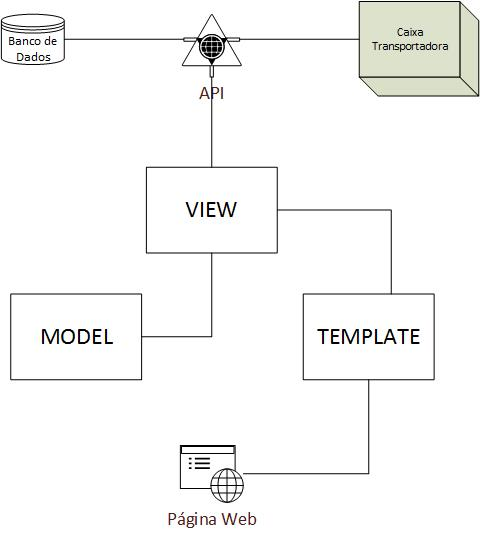
\includegraphics[width=16cm]{figuras/arquitetura_software.jpg}
\caption{Arquitetura de Software}
\end{figure}

\subsubsection{Integração}

	A integração com as outras áreas de engenharias deste projeto consiste na comunicação do sistema interno e webapp com os dispositivos eletrônicos e sensoriamento disposto na caixa transportadora. O sistema interno está atuando em conjunto com o microcontrolador para recepção dos dados dos sensores de temperatura, trava e controle on/off, e com a raspberry pi para transmissão dos dados para a API, com isso a equipe de desenvolvimento de software está a trabalhar ativamente com a equipe de eletrônica a fim de atingir os objetivos específicos relacionados à esses temas.

\subsection{Requisitos Implementados}
\subsubsection{Cadastro de Usuários}
	Foi implementado um sistema de cadastro de usuários, aos quais estes serão classificados e cadastrados em três diferentes tipos de acordo com seu nível de autorização.

\begin{itemize}
\item Administrador: Terá controle total sobre a aplicação; somente usuário administrador terá acesso aos cadastros de usuários e novas câmaras de transporte;
\item Transportador:  Terá autorização para iniciar um novo transporte e visualizar o andamento do mesmo;
\item Usuário: Poderá apenas visualizar as informações de um transporte em andamento.
\end{itemize}

	Para o cadastro serão necessários informar os dados de nome de usuário, email, senha e nível de acesso. A seguir a tela de cadastro:

\begin{figure}[H]
\centering
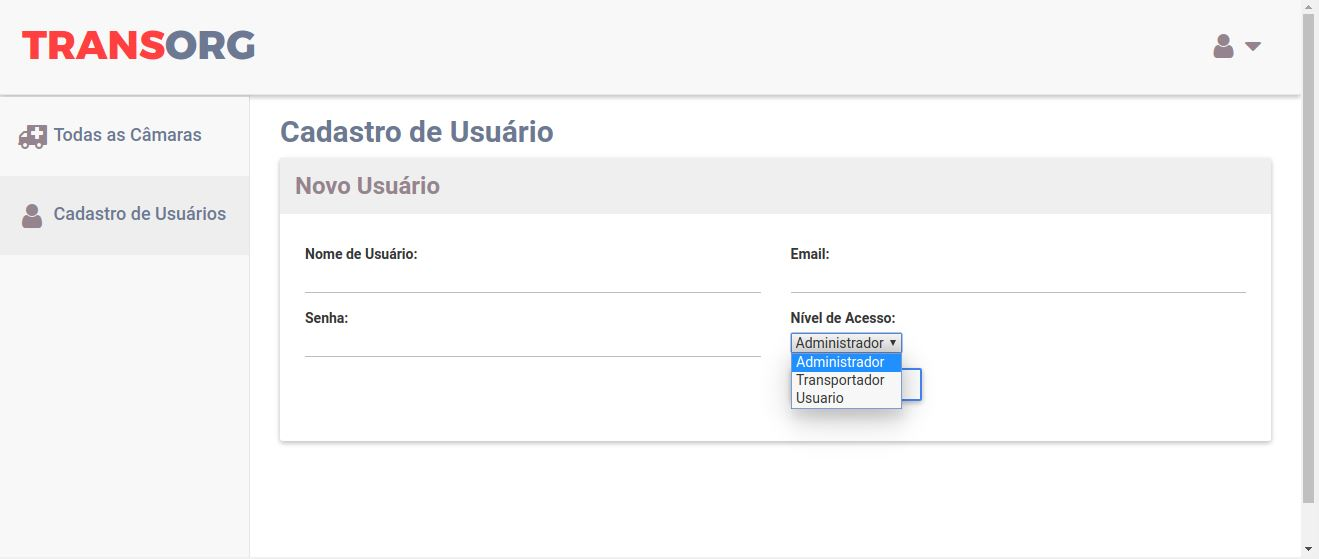
\includegraphics[width=16cm]{figuras/cadastro_software.jpg}
\caption{Arquitetura de Software}
\end{figure}

\subsubsection{Listar e Apagar Usuários}
	O sistema irá dispor de uma página específica para listar todos os usuários cadastrados juntamente com a opção de deletar os mesmos. A seguir a tela de listagem de usuários:

\begin{figure}[H]
\centering
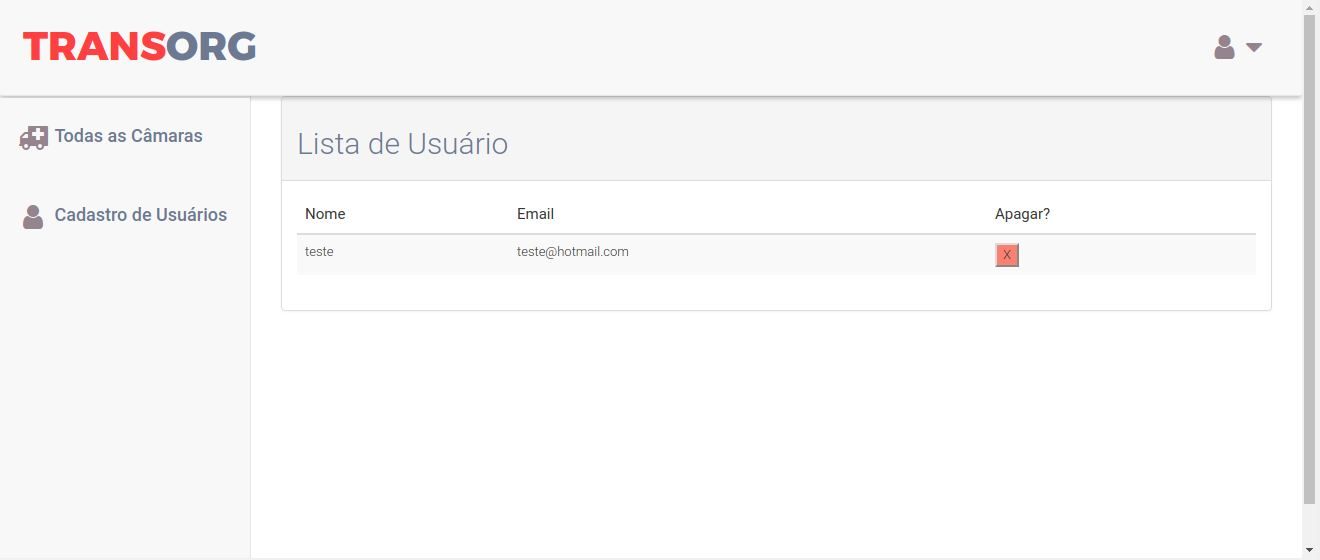
\includegraphics[width=16cm]{figuras/listaUsuarios_software.jpg}
\caption{Listar usuários}
\end{figure}

\subsubsection{Sistema de Login}
	O sistema de autenticação se dará por meio do envio dos dados das credenciais à API, composto por nome de usuário e senha, e caso estas informações estejam corretas a API retorna um token de acesso ao qual é guardado em uma sessão, onde para acesso às páginas, o sistema sempre verificará se consta na sessão o token correto, caso contrário retornará à página de login. 
	
	A seguir a tela de Login:

\begin{figure}[H]
\centering
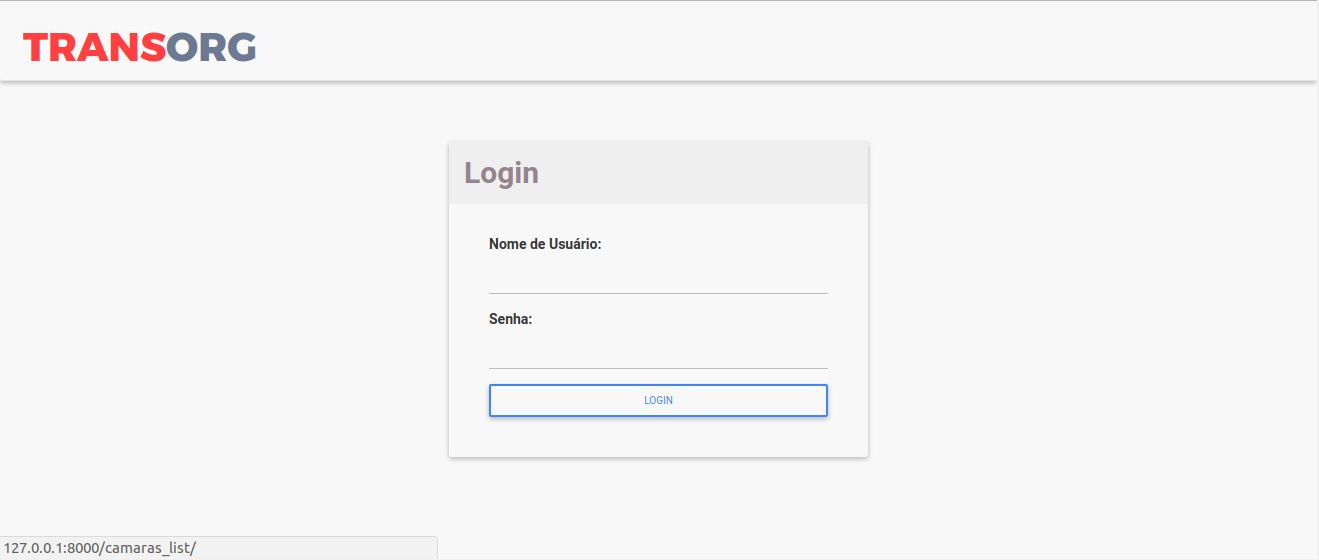
\includegraphics[width=16cm]{figuras/login_software.jpg}
\caption{Login no WebApp}
\end{figure}

\subsubsection{Cadastro de Câmaras}
	O sistema dispõe de um cadastro de novas câmaras, onde é solicitado o nome da mesma para seu cadastro. Internamente é criada junto ao webservice com seu id relacionado. A partir de sua criação, esta câmara já fica disponível para transporte no sistema.
	
	A seguir a tela de cadastro de câmaras:

\begin{figure}[H]
\centering
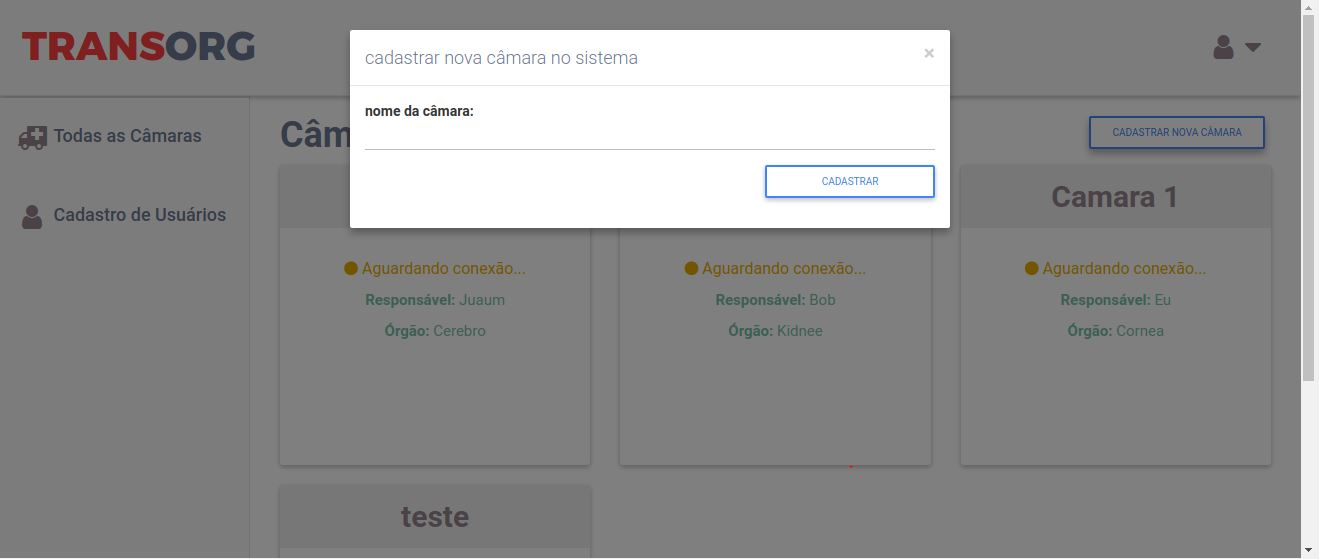
\includegraphics[width=16cm]{figuras/cadastroCamaras_software.jpg}
\caption{Cadastro de Câmaras}
\end{figure}

\subsubsection{Visualizar Todas as Câmaras}
	A tela principal do sistema se dará pela visualização das câmaras disponíveis e em uso, a partir dela será possível iniciar novas solicitações de transporte. Câmaras disponíveis e fora de uso também há a opção de deleção.
	
	A seguir tela de visualização de câmaras:

\begin{figure}[H]
\centering
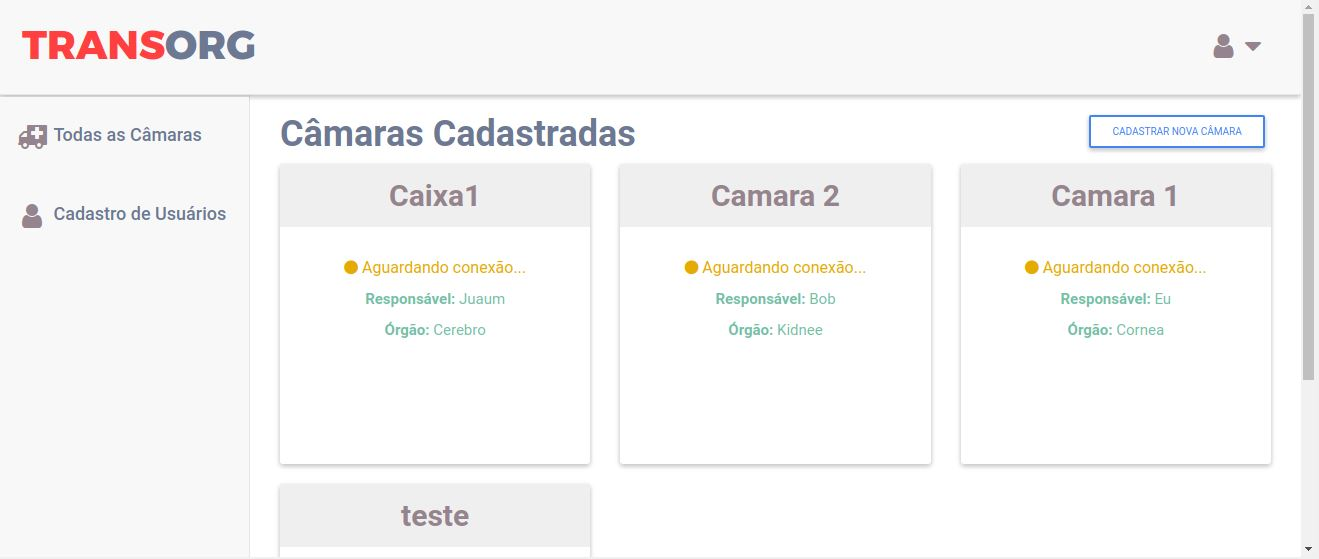
\includegraphics[width=16cm]{figuras/listaCamaras_software.jpg}
\caption{Listar Câmaras}
\end{figure}

\subsubsection{Iniciar Novo Transporte:}
	A partir da seleção de uma câmara disponível o usuário é redirecionado à página de início de um novo transporte onde é solicitado informar o responsável pelo transporte e o órgão ao qual será transportado.
	
	A seguir a tela de início de um novo transporte:

\begin{figure}[H]
\centering
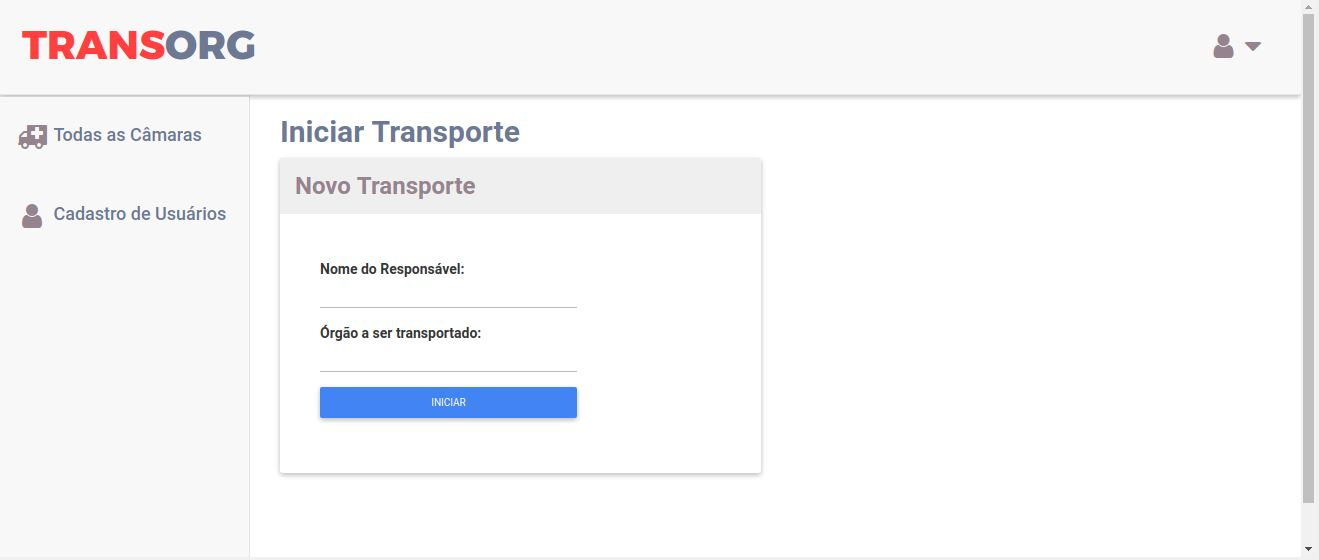
\includegraphics[width=16cm]{figuras/iniciarTransporte_software.jpg}
\caption{Iniciar Transporte}
\end{figure}

\subsubsection{Visualizar Transporte em Andamento:}
	A principal funcionalidade do sistema, onde se é possível visualizar todas as informações de um transporte em andamento. As informações apresentadas são: gráfico de temperatura, temperatura atual, localização atual, responsável pelo transporte, órgão transportado, status da trava de segurança e data e hora destes dados.

	A seguir tela de visualização de andamento de um transporte ativo:

\begin{figure}[H]
\centering
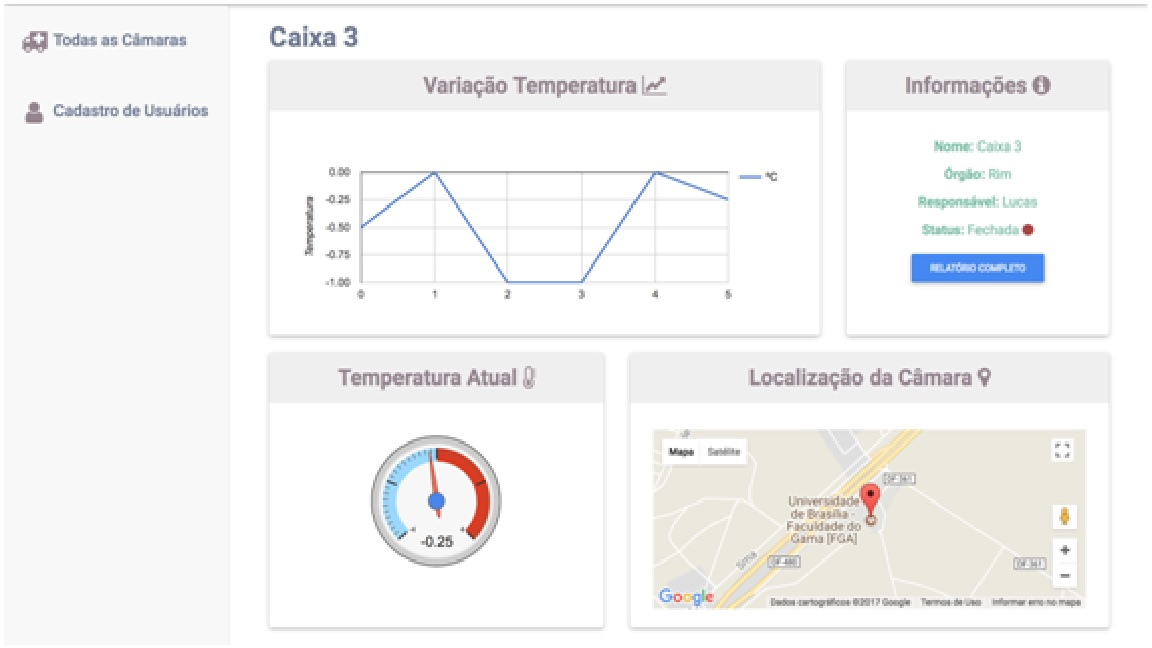
\includegraphics[width=16cm]{figuras/camara_software.jpg}
\caption{Câmara de transporte}
\end{figure}

\subsubsection{Relatório}
	O sistema dispõe de uma funcionalidade de relatório, ao qual o usuário irá visualizar as informações dos transportes realizados, com opção de exportação em PDF.
	A seguir tela de relatório:
\begin{figure}[H]
\centering
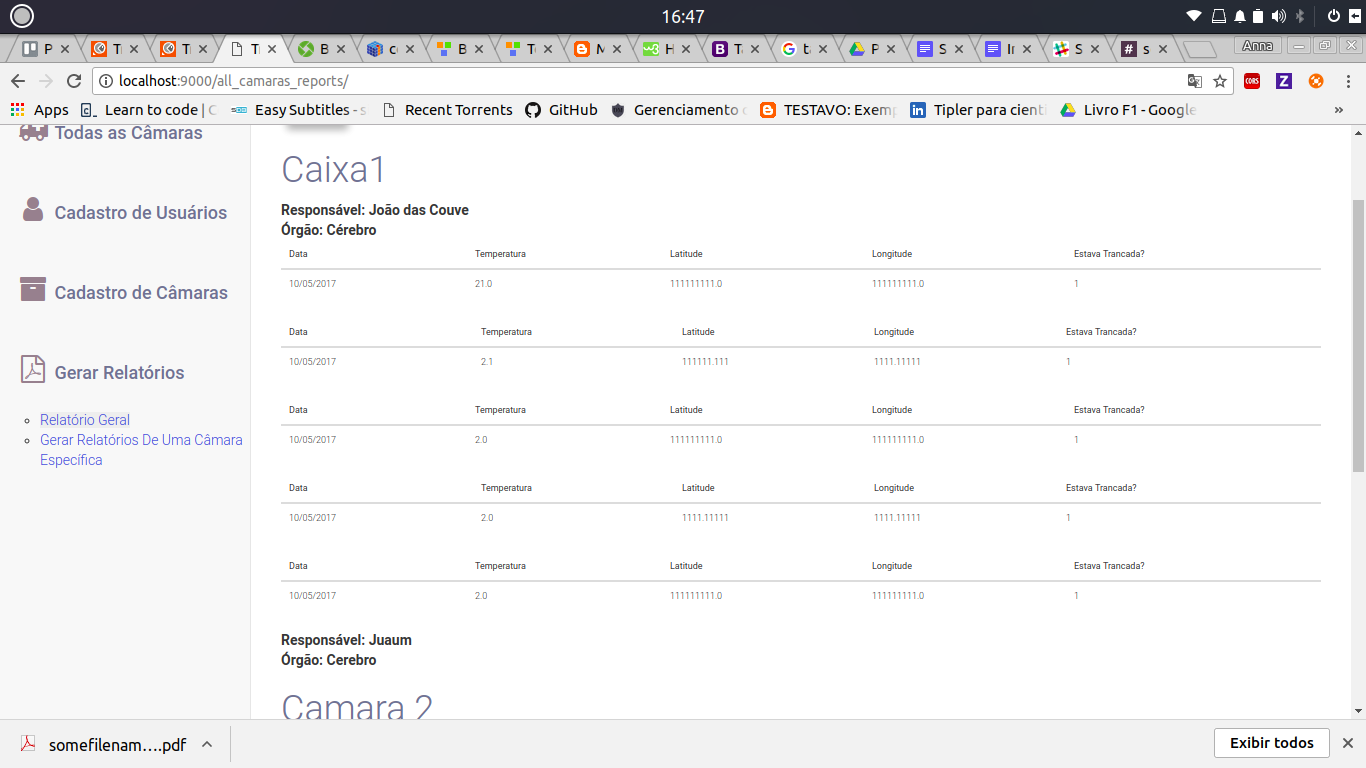
\includegraphics[width=16cm]{figuras/relatorio_software.png}
\caption{Relatórios do sistema}
\end{figure}

\subsubsection{API}

A API é o intermediário entre os sistemas e o banco de dados, uma forma de garantir que todos os dados sejam inseridos e recuperados através de um sistema em comum. Dessa forma podemos trabalhar com qualquer meio de visualização de dados e métodos de inserção, que se torna imprescindível para o funcionamento de um sistema onde temos uma interface WEB e um equipamento eletrônico que irá inserir dados no banco de dados.

A caixa transportadora acessará a API para fornecer as leituras dos sensores de localização, temperatura, fechamento e os dados do transporte. A API tratará de armazenar esses dados no banco através dos endpoints configurados. A partir daí o sistema WEB pode recuperar esses dados com chamadas nos endpoints da API. 

Portanto a caixa transportadora servirá somente como interface de inserção de dados enquanto o WEB app funcionará como inserção e recuperação.

A API foi documentada na plataforma POSTMAN que automatiza e testa os endpoints configurados. 

 A seguir a tela da ferramenta com a api configurada:

\begin{figure}[H]
\centering
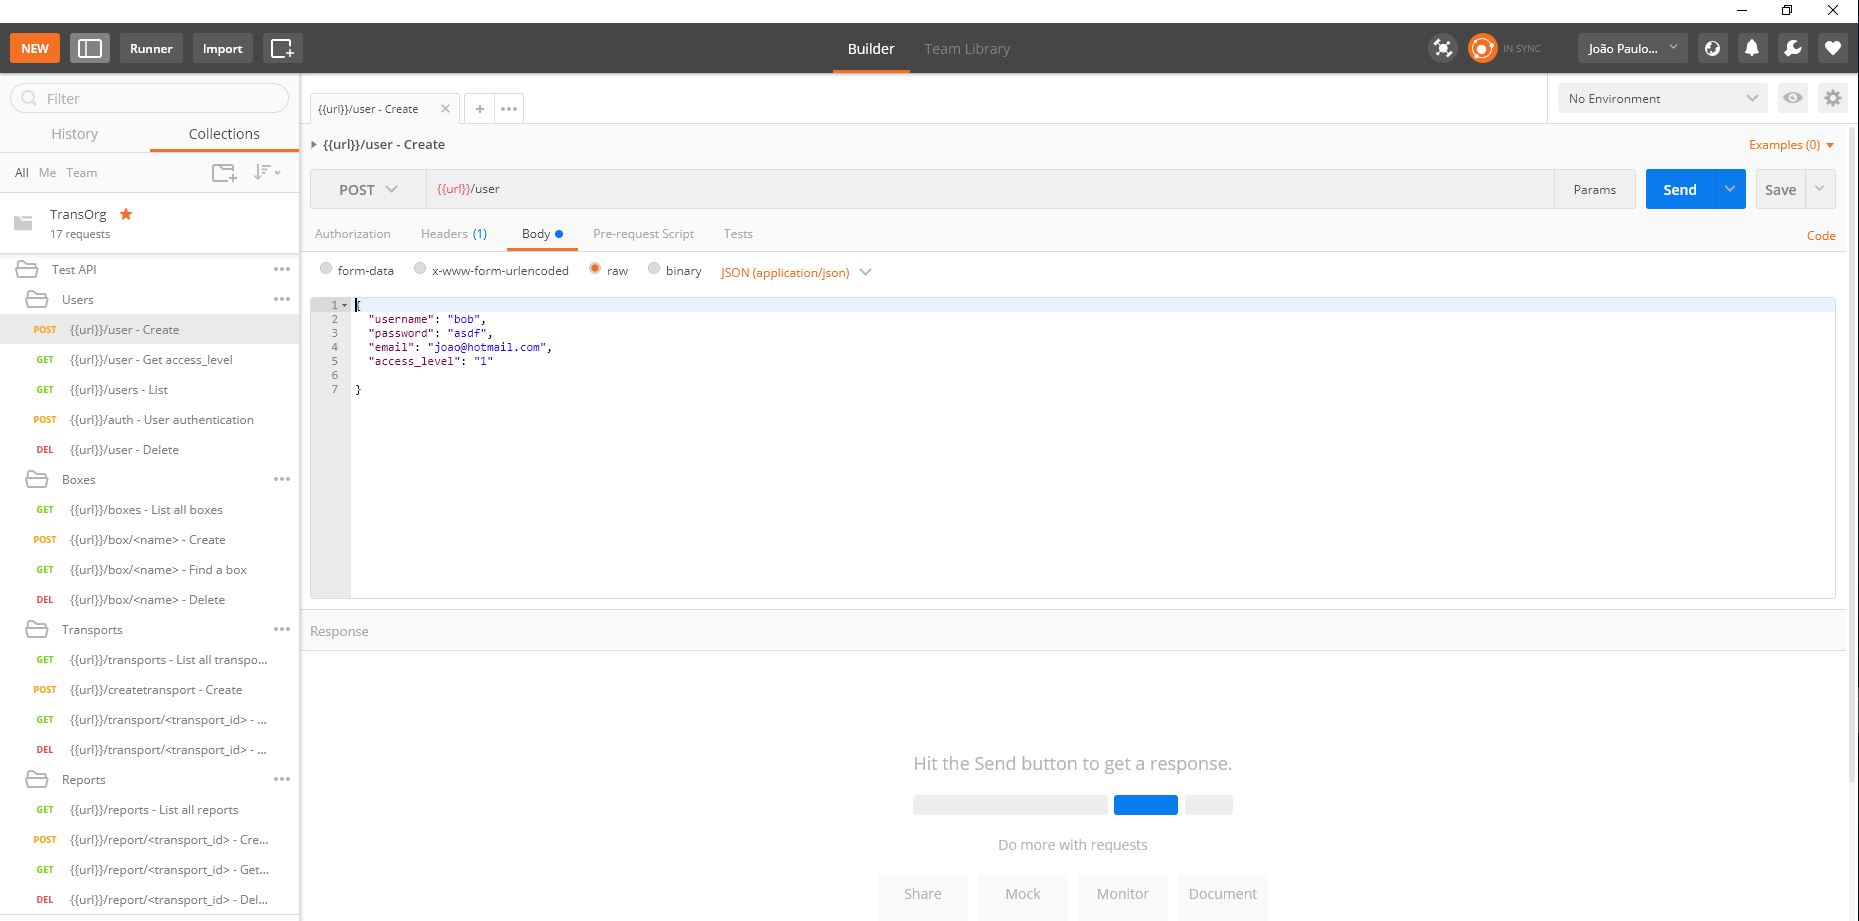
\includegraphics[width=16cm]{figuras/api_software.jpg}
\caption{API do Sistema}
\end{figure}